\section{Metodología}
\begin{multicols}{2}
    [ Esta es una prueba de \LaTeX para la charla con los MLSA $<3$]
    \blindtext
\end{multicols}
\lipsum[1]

Quiero referencia mi matrix \ref{matrix}, ahora mi fracción \ref{mifraccion}
\begin{figure}
    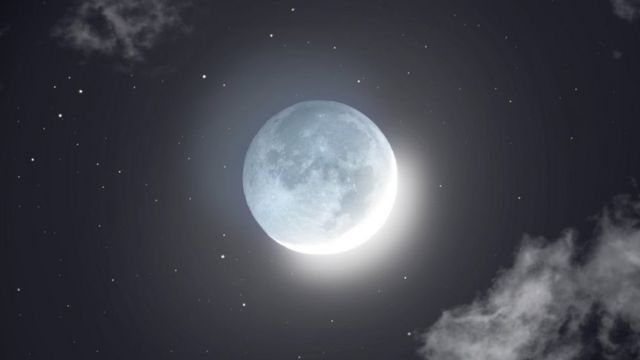
\includegraphics[width=\linewidth]{build/img/luna.jpg}
\end{figure}

\begin{table}[]
    \begin{tabular}{|c|c|c|c|c|}
    \hline
    \textbf{Números} & \textbf{rf} & \textbf{gr} & \textbf{fg} & \textbf{5}  \\ \hline
    \textbf{1}       & \textbf{2}  & \textbf{3}  & \textbf{4}  & \textbf{5} \\ \hline
    \textbf{4}       & \textbf{5}  & \textbf{6}  & \textbf{7}  & \textbf{7} \\ \hline
    \textbf{7}       & \textbf{6}  & \textbf{5}  & \textbf{34} & \textbf{6} \\ \hline
    \end{tabular}
    \end{table}

\begin{equation} \label{matrix}
    \begin{bmatrix}
        3&3  & 4\\ 
        4& 5 & 5\\ 
        6& 65 & 5
    \end{bmatrix}    
\end{equation}
\begin{equation} \label{mifraccion}
   \left( \frac{2}{4}x + \frac{7}{8}\right)x=0   
\end{equation}

